\documentclass{beamer}
\usepackage{amsmath}
\usepackage{tikz}
\usepackage{graphicx}
\usepackage{xcolor}
\usepackage{soul}
\usepackage{acronym}
\usepackage{hyperref} 
\usetikzlibrary{overlay-beamer-styles}
\usetikzlibrary{shapes, positioning, calc}
\usetikzlibrary{decorations.text}
\usetikzlibrary{shapes.geometric, arrows}

\tikzstyle{data} = [circle, draw=black]
\tikzstyle{arrow} = [-stealth]

\usetheme{Frankfurt}

\title{Beamer Presentation}
\author{Abdus Samee}
\date{\today}

\begin{document}

\maketitle

\begin{frame}
    \frametitle{Points}
    \begin{description}
        \item[ONE] $a^2+b^2$ \pause
        \item[TWO] $a^2-b^2$ \pause
        \item[THREE] $a^3+b^3$ \pause
        \item[FOUR] $a^3-b^3$ \pause
        % \st{Strike through text..}
    \end{description}
\end{frame}

\begin{frame}{More Bullet Points}
    \begin{itemize}
        \item[$\bullet$]<1-> \textbf{First Point}
        \item[$\triangle$]<2-> \textbf{Second Point}
        \item<3-> \textbf{Third Point}
    \end{itemize}
\end{frame}

\begin{frame}
    \frametitle{Tikz Figure}
    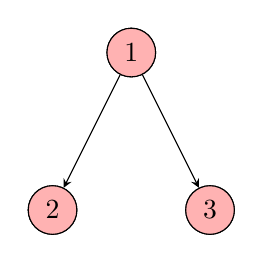
\begin{tikzpicture}[node distance = 2cm]
        \node (a) [data] {1};
        \node (b) [data, below of=a, xshift=-1cm] {2};
        \node (c) [data, below of=a, xshift=1cm] {3};
    
        \draw[arrow] (a) -- (b);
        \draw[arrow] (a) -- (c);
        \pause

        \node (a) [data, fill=red!30] {1}; \pause
        \node (b) [data, below of=a, xshift=-1cm, fill=red!30] {2}; \pause
        \node (c) [data, below of=a, xshift=1cm, fill=red!30] {3};
    \end{tikzpicture}
\end{frame}

\begin{frame}
    \frametitle{Yet another Tikz Figure}
    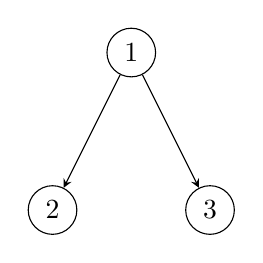
\begin{tikzpicture}[node distance=2cm]
        \node (a) [data] {1};
        \node (b) [data, below of=a, xshift=-1cm] {2};
        \node (c) [data, below of=a, xshift=1cm] {3};
        \pause
    
        \draw[arrow] (a) -- (b); \pause
        \draw[arrow] (a) -- (c); \pause
    \end{tikzpicture}
\end{frame}

\begin{frame}{Column Picture}
    \begin{columns}
        \column{.5\textwidth}
        
        \includegraphics[height=.85\textheight, width=.85\textwidth]{pic.jpg}
        \column{.5\textwidth}
        
        \textbf{A Minecraft Image}
    \end{columns}
\end{frame}

\begin{frame}{Column Text}
    \begin{columns}
        \column{.5\textwidth}
        \color{red} % can use \textcolor{red}{my_text} too...
        $a^2+b^2$ \pause \\
        $a^2-b^2$ \pause

        \column{.5\textwidth}
        \color{blue}
        $a^3+b^3$ \pause \\
        $a^3-b^3$
    \end{columns}
\end{frame}

\begin{frame}{Callout Pointer}
    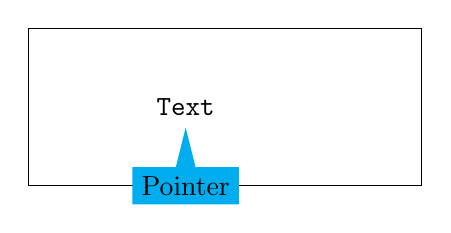
\begin{tikzpicture}
        \draw (1,2) rectangle (6,4); \pause
        \node (a) at (3,3) {\texttt{Text}}; \pause
        \node[rectangle callout, color=black, fill=cyan, callout relative pointer={(0,0.5)}, below of=a] {Pointer};
    \end{tikzpicture}
\end{frame}

\begin{frame}
\label{table}
\frametitle{Table Onslide Animation}
    \begin{table}
        \begin{tabular}{l | c | c | c | c }
            Competitor Name & Swim & Cycle & Run & Total \\
            \hline \hline
            John T & 13:04 & 24:15 & 18:34 & 55:53 \onslide<2-> \\ 
            Norman P & 8:00 & 22:45 & 23:02 & 53:47 \onslide<3->\\
            Alex K & 14:00 & 28:00 & n/a & n/a \onslide<4->\\
            Sarah H & 9:22 & 21:10 & 24:03 & 54:35 
        \end{tabular}
        \caption{Triathlon results}
    \end{table}
\end{frame}

% \begin{frame}{Acronyms}
%     \begin{acronym}
%         \acro{CSE}{Computer Science & Engineering}
%     \end{acronym}
% \end{frame}

\begin{frame}[fragile]{Code}
    \begin{semiverbatim}
        \\begin\{frame\}
        \\includegraphics\{fig.jpg\}
        \\end\{frame\}
    \end{semiverbatim}
\end{frame}

\begin{frame}{Buttons}
    \hyperlink{table}{\beamerbutton{Table Animation}}
\end{frame}

\begin{frame}{Yet another Tikz Picture}
    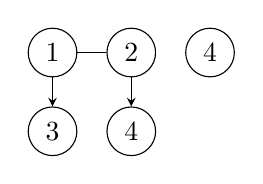
\begin{tikzpicture}
        \node (a) [data] {1};
        \node (b) [data, right of=a] {2};
        \node (c) [data, below of=a] {3};
        \node (d) [data, right of=b, visible on=<-2>] {4};

        \draw[arrow] (a) -- (c);
        \draw (a) -- (b);
        \draw[dotted] (b) -- (d); \pause

        \draw[thick, color=white] (b) -- (d);\pause
        \node (d1) [data, below of=b] {4};
        \draw[arrow] (b) -- (d1);
    \end{tikzpicture}
\end{frame}

\end{document}
